\begin{figure}[tbp]
\centering
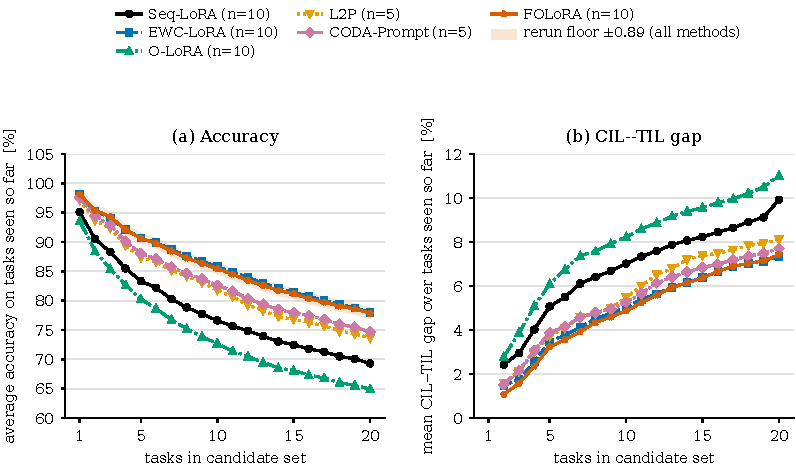
\includegraphics[width=0.92\linewidth]{figures/forgetting_curve_cifar100.pdf}
\caption{Average accuracy over the candidate classes seen so far (left) and the mean
CIL--TIL gap over those candidate sets (right) on Split CIFAR-100. Every point is a single
feature extraction of the \emph{terminal} model re-scored against a growing candidate set;
the horizontal axis is the number of tasks in that candidate set ($1$ to $20$, i.e.\ $5$ to
$100$ candidate classes at $5$ classes per task), not training time, so the leftmost point
already contains the forgetting incurred over the whole sequence. Each curve is drawn at the configuration \emph{and} the seed budget of its row in
Table~\ref{tab:main} --- ten seeds for Seq-LoRA, EWC-LoRA, O-LoRA and FOLoRA, five for L2P
and CODA-Prompt --- so its right-hand endpoint reproduces that row's
$\overline{\mathrm{ACC}}$. Six of the eight rows of Table~\ref{tab:main} are plotted;
InfLoRA and the SimpleCIL floor are tabulated but not drawn here, so the legend and the
table do not cover an identical row set. Those budgets differ between methods (Sec.~\ref{sec:setup}), so
the legend carries each curve's $n$ and the figure implies no equal $n$. No smoothing or
interpolation is applied --- the markers are the per-task measurements. The shaded band is
the run-to-run resolution of this measurement ($\pm0.89$ points, i.e.\ the standard deviation
of the difference between two independent runs of one configuration;
Sec.~\ref{sec:discussion}) --- a property of the protocol rather than of any one method, and
it applies to every curve shown. The vertical axis is bounded below at $60$, i.e.\ $4.94$
points under the lowest value plotted, rather than at zero; the full range is
$60$--$105$.}
\label{fig:curve-cifar}
\end{figure}

\begin{figure}[tbp]
\centering
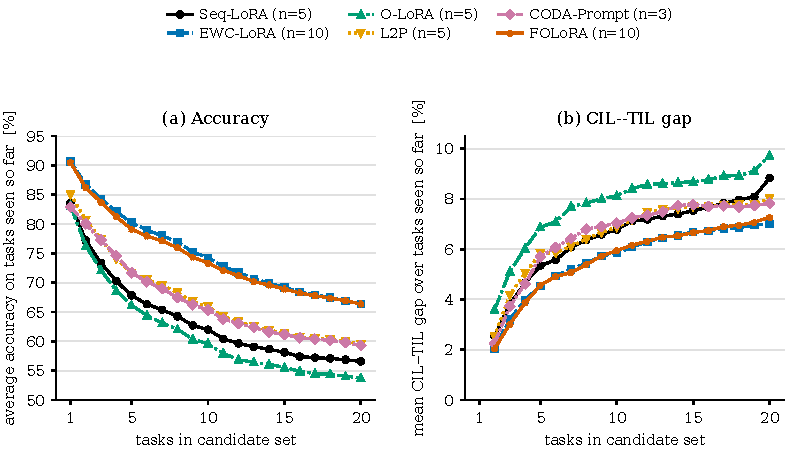
\includegraphics[width=\linewidth]{figures/forgetting_curve_imagenetr.pdf}
\caption{Average accuracy over the candidate classes seen so far (left) and the mean
CIL--TIL gap over those candidate sets (right) on Split ImageNet-R. As in
Fig.~\ref{fig:curve-cifar}, each point is a single feature extraction of the terminal model
re-scored against a growing candidate set --- the number of tasks in it, $1$ to $20$, i.e.\
$10$ to $200$ candidate classes at $10$ classes per task --- not a training trajectory. Each curve is drawn at the configuration \emph{and} the seed budget of
its row in Table~\ref{tab:main} --- CODA-Prompt on three seeds, L2P, O-LoRA and Seq-LoRA on
five, EWC-LoRA and FOLoRA on ten --- so its right-hand endpoint reproduces that row's
$\overline{\mathrm{ACC}}$. As in Fig.~\ref{fig:curve-cifar}, six of the eight rows of
Table~\ref{tab:main} are plotted; InfLoRA and the SimpleCIL floor are tabulated but not
drawn. Those budgets differ between methods (Sec.~\ref{sec:setup}), so
the legend carries each curve's $n$ and the figure implies no equal $n$. No
reproducibility-floor band is drawn, because that floor was measured on CIFAR-100 only and
we do not transfer it to another dataset. The vertical axis is bounded below at $50$, i.e.\
$3.72$ points under the lowest value plotted.}
\label{fig:curve-inr}
\end{figure}
